Il periodo di verifica e validazione inizia con la consegna della RQ e termina con la consegna della RA.\newline
Durante questo periodo, sono svolte le seguenti attività:
\begin{itemize}
	\item \textbf{Modifica e incremento}: all'inizio  del  periodo  vengono  modificati  e  verificati  i seguenti documenti seguendo le indicazioni risultanti dalla \RQ{}:
	\begin{itemize}
		\item \textbf{Piano di progetto};
		\item \textbf{Piano di qualifica};
		\item \textbf{Norme di progetto};
		\item \textbf{Manuale Utente}: questa attività consta nel miglioramento del manuale utente completandolo inserendo tutte le funzionalità offerte dall'applicativo;
		\item \textbf{Manuale Sviluppatore};
		\item \textbf{Product Baseline};
	\end{itemize}
	\item \textbf{Glossario}: il documento viene ampliato inserendo nuovi termini;
	\item \textbf{Codifica}: si conclude l'implementazione delle funzionalità espresse dai requisiti obbligatori, e si implementano alcuni requisiti desiderabili.
	\item \textbf{Validazione e Collaudo}: queste attività consistono nell'esecuzione di ulteriori test e miglioramenti del prodotto al fine di accertare che tutti i vincoli qualitativi e i requisiti siano rispettati (conci.
\end{itemize}
Il numero di incrementi per realizzare tali attività ha un valore fissato a 4.
Il progetto cresce in modo incrementale da un'iterazione alla successiva, adattandosi ai requisiti, in modo evolutivo, sulla base del feedback delle iterazioni precedenti, tra cui la valutazione della \RQ{}.
\begin{figure}[H]
		\hspace*{-1.5cm}
	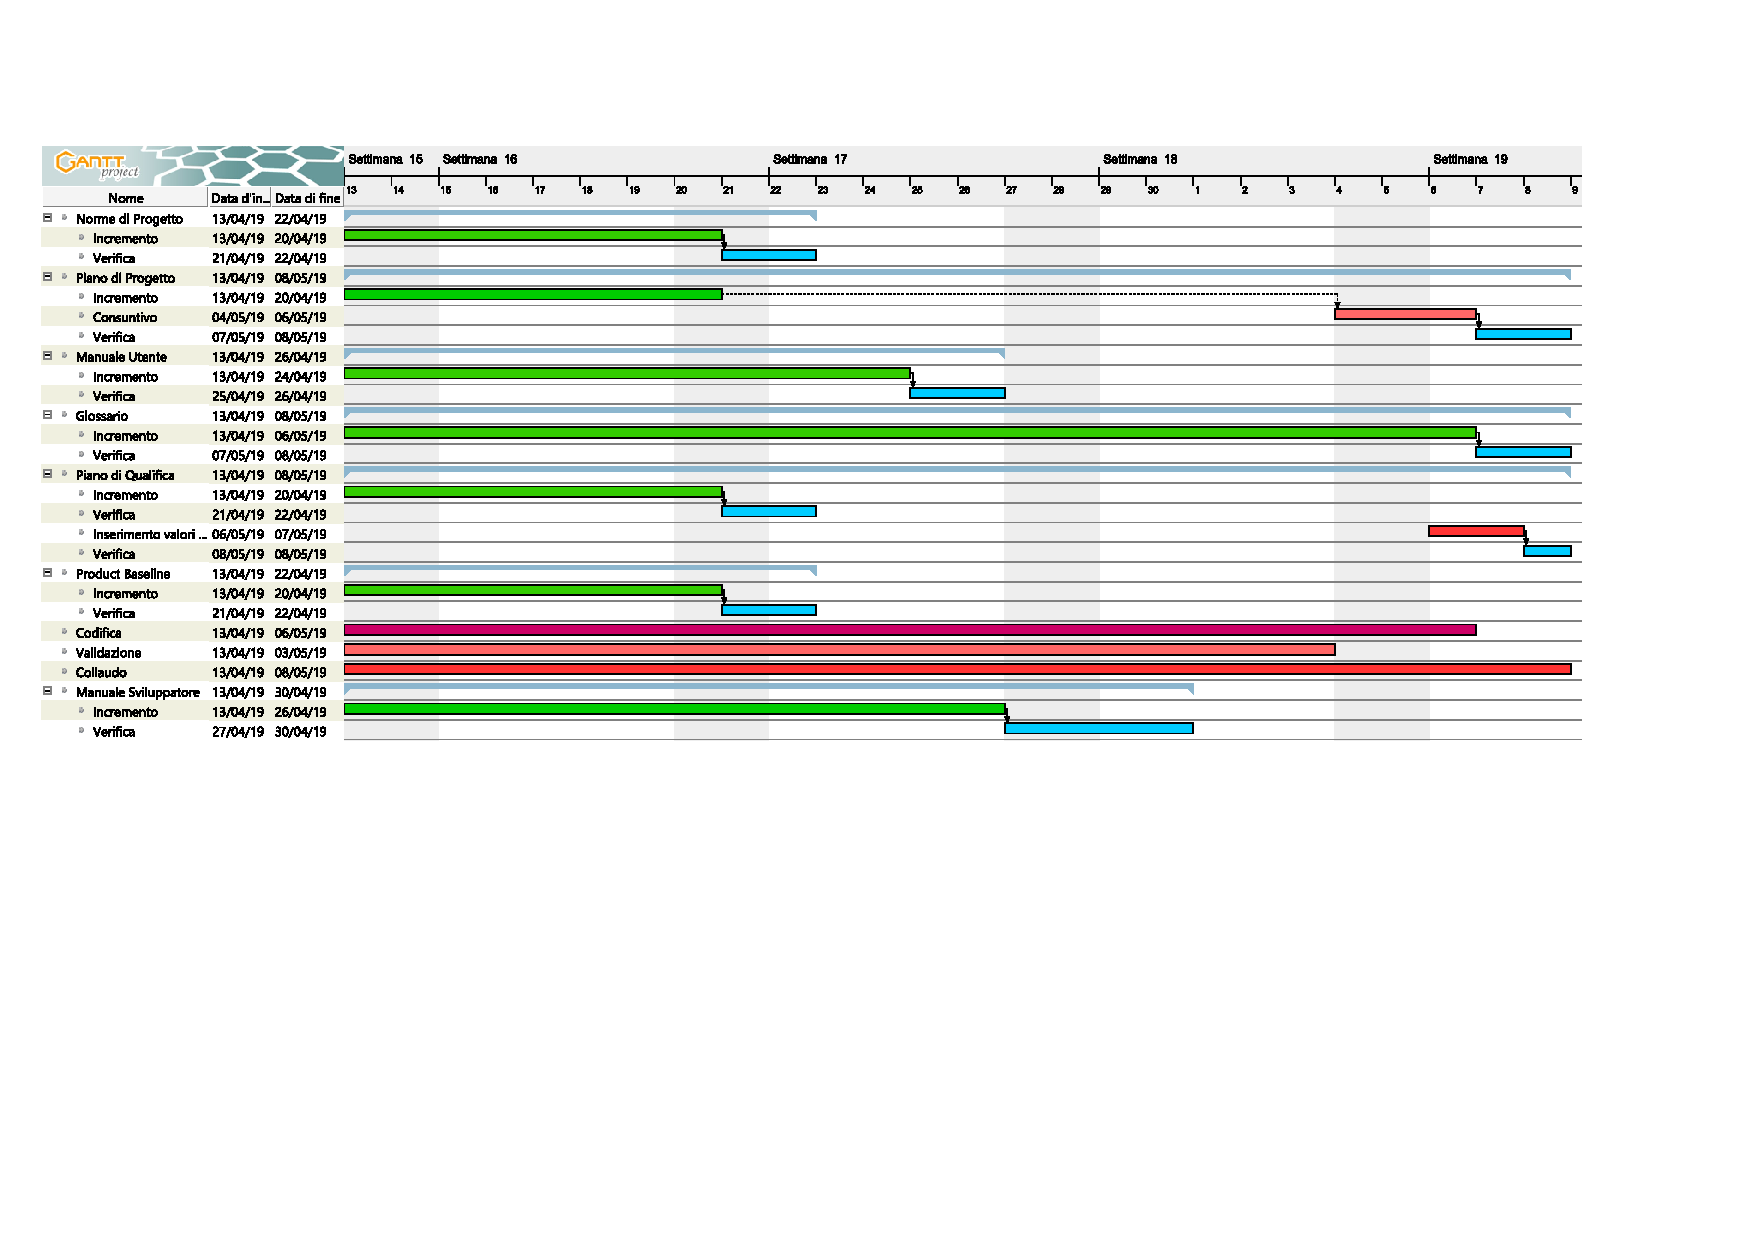
\includegraphics[width=19.4cm, height=8cm]{Pianificazione/verificaValidazione.pdf}
	\caption{Diagramma di Gantt del periodo di verifica e validazione}
\end{figure}